\chapter{Results}
\label{sec:results}

\section{Findings from the Simulations}
- Wie in Vorversuchen schon bemerkt: QE-Schema produziert numerische Fehler, die sich darin zeigen, dass Preise mehrfach in der Simulation vorkommen. Bei korrekter Simulation ist der häufigste Preis im ersten Pfad im einstelligen Bereich, bei Fehlern im Hunderter- oder Tausenderbereich.
- Abbildung \ref{fig:max_number_of_same_prices_distribution} zeigt die Verteilung, man sieht einen Peak bei 1, was darauf hindeutet, dass die meisten Simulationen korrekt sind. Man sieht aber auch, dass es einige Simulationen gibt, wo der selbe Preis bis zu 250000 mal vorkommt, hier kam es zu numerischen Fehlern. Bei diesen Simulationen stellt man fest, dass, wenn es das erste Mal zu numerischen Fehlern kommt, der Rest der Zeitreihe den selben Preis hat. Bei Simulationen mit 250000 gleichen Preises kam es also sehr früh in der Zeitreihe zu einem numerischen Fehler.

\begin{figure}
    \centering
    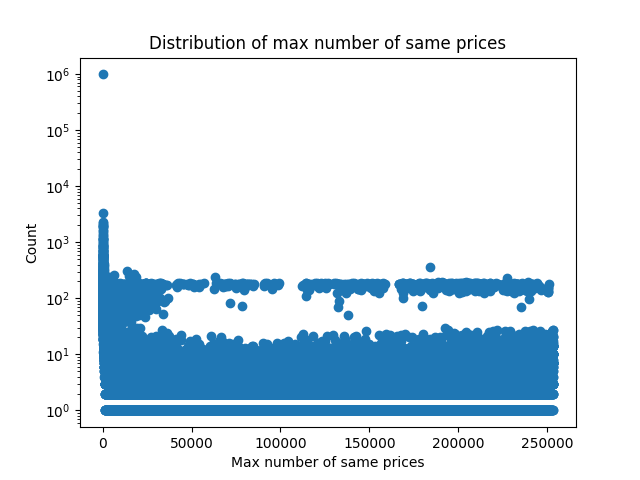
\includegraphics[width=0.8\textwidth]{img/max_number_of_same_prices_distribution.png}
    \caption{Distribution of the maximum number of the same prices in the first path of the simulation}
    \label{fig:max_number_of_same_prices_distribution}
\end{figure}

- Für die weitere Untersuchung sollen solche Simulationen ausgeschlossen werden, da sie nicht korrekt sind. Da es durchaus möglich ist, dass es auch bei korrekter Simulation zu gleichen Preisen kommt, wird ein Schwellwert gesucht, sodass möglichst viele korrekte Simulationen in der Untersuchung bleiben. Abbildung \ref{fig:max_number_of_same_prices_cumulative_percentage} zeigt für verschiedene Schwellwerte (die maximale Anzahl an gleichen Preisen) den kumulativen Anteil der Simulationen, die diesen Schwellwert nicht überschreiten. Wählt man den Schwellwert 1, also nur Simulationen, bei denen nie ein Preis mehrfach vorkommt, verbleiben bleiben 68.40\% der Simulation. Je höher man den Schwellwert setzt, desto weniger Simulationen fallen weg, aber unter Umständen verbleiben auch Simulationen, die numerische Fehler enthalten. Das betrifft aber nur sehr wenige Simulationen, der Anteil an inkludierten Simulationen steigt fast gar nicht. Für die späteren Untersuchungen werden also alle Simulationen entfernt, bei denen der selbe Preis mehr als einmal vorkommt.

\begin{figure}
    \centering
    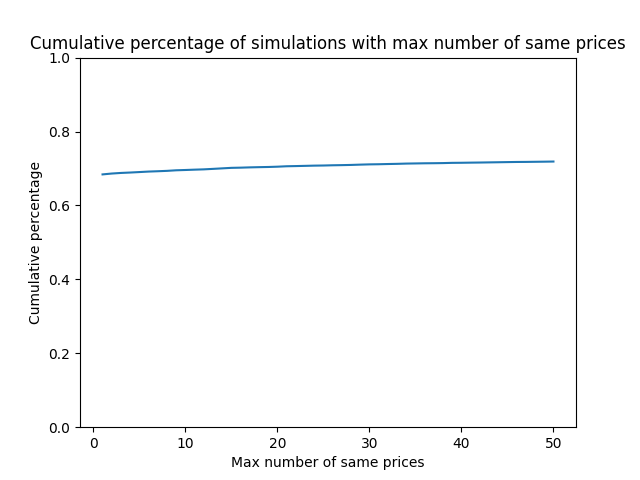
\includegraphics[width=0.8\textwidth]{img/max_number_of_same_prices_cumulative_percentage.png}
    \caption{Cumulative percentage of simulations that do not exceed the maximum number of same prices}
    \label{fig:max_number_of_same_prices_cumulative_percentage}
\end{figure}

\begin{figure}
    \centering
    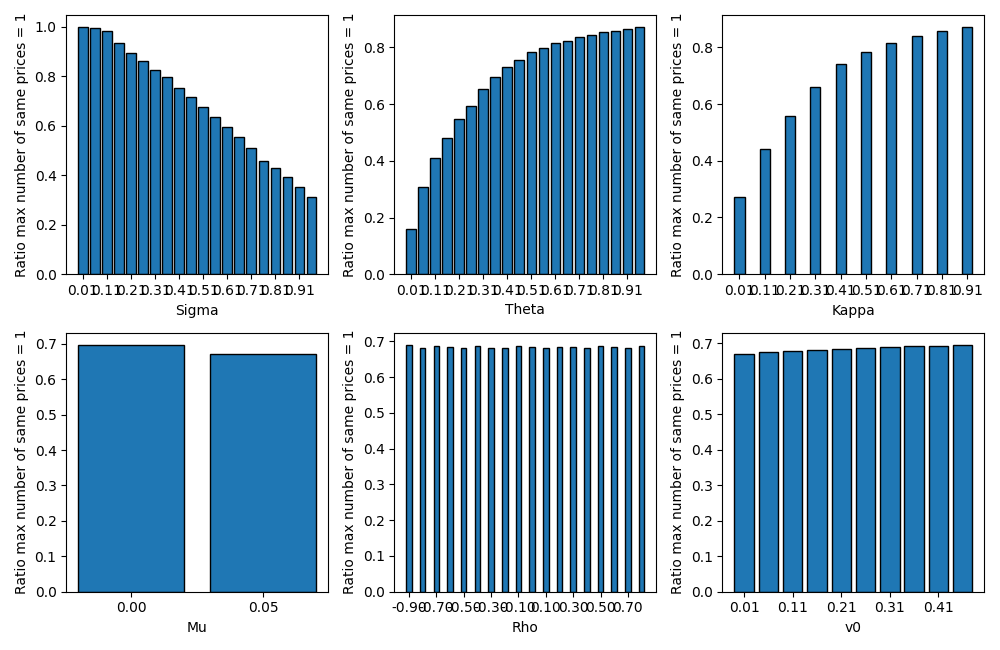
\includegraphics[width=0.8\textwidth]{img/max_number_of_same_prices_ratio_parameters.png}
    \caption{Ratio of simulations that do not exceed the maximum number of same prices in relation to the parameters of the Heston model}
    \label{fig:max_number_of_same_prices_ratio_parameters}
\end{figure}

\begin{figure}
    \centering
    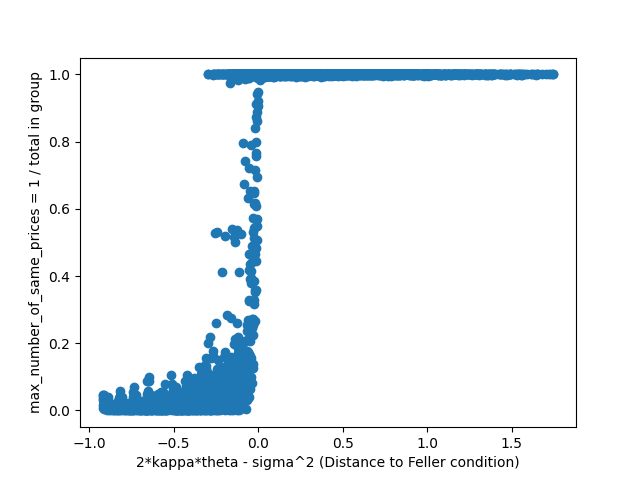
\includegraphics[width=0.8\textwidth]{img/max_number_of_same_prices_ratio_feller_diff.png}
    \caption{Ratio of simulations that do not exceed the maximum number of same prices in relation to the value $D$}
    \label{fig:max_number_of_same_prices_ratio_D}
\end{figure}

- Untersuchung, woher diese Fehler kommen: Dazu bestimmen des Anteils der Simulationen, die korrekt in Abhängigkeit eines jeden einzelnen Parameters des Heston-Modells (siehe Abbildung \ref{fig:max_number_of_same_prices_ratio_parameters}). Man erkennt, dass mit zunehmendem $\sigma$ die Fehler zunehmen, während mit zunehmendem $\theta$ und $\kappa$ die Fehler abnehmen. Die Parameter $\mu$, $\rho$ und $v_0$ haben keinen Einfluss auf die Fehlerhäufigkeit. Das legt nahe, dass die Fehler mit der Feller condition zusammenhängen. Deshalb untersuche ich nun die Fehlerhäufigkeit und den Wert $D = 2\kappa\theta - \sigma^2$. Ist dieser Wert positiv, so ist die Feller condition erfüllt, je negativer er ist, desto weniger erfüllt ist die Feller condition. Abbildung \ref{fig:max_number_of_same_prices_ratio_D} zeigt, dass, sobald die Feller condition nicht mehr erfüllt ist, die Fehlerhäufigkeit stark zunimmt. Wenn die Feller condition erfüllt ist, so sind 99.90\% der Simulationen korrekt, ist die Feller condition nicht erfüllt, so sind es nur 25.48\%. Insgesamt erfüllen 57.80\% der Simulationen die Feller condition.
- Im Folgenden werden einige Expansionsmethoden weiter untersucht, gestartet wird mit der Gram-Charlier-Expansion, da sie die einfachste Methode ist.

\section{Investigating the Results for the Gram-Charlier-Expansion}

\subsection{Comparing with the Kolmogorov-Smirnov-Test}

\begin{figure}
    \centering
    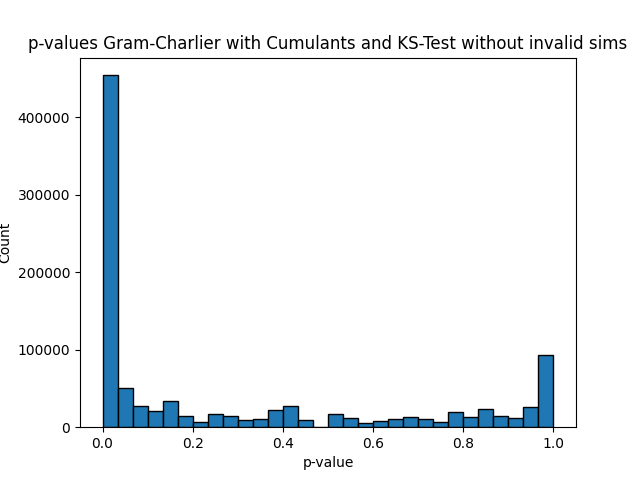
\includegraphics[width=0.8\textwidth]{img/GC_cum_KS_p_value_histogram.png}
    \caption{Distribution of p values of the Kolmogorov-Smirnov-Test for the Gram-Charlier Expansion with Cumulants vs the theoretical density without invalid simulations}
    \label{fig:GC_cum_KS_p_value_histogram}
\end{figure}

- In Abbildung \ref{fig:GC_cum_KS_p_value_histogram} sieht man die Verteilung der p values des Kolmogorov-Smirnov-Tests für die Gram-Charlier Expansion mit Kumulanten im Vergleich zur theoretischen Dichte. Dabei wurden alle Simulationen entfernt, bei denen der selbe Preis mehr als einmal vorkommt. Ein p Wert von über 5\% bedeutet, dass es keine signifikanten Unterschiede zwischen den beiden Verteilungen gibt, die Gram-Charlier Expansion auf Basis von Kumulanten approximiert die theoretische Dichte also gut genug. Man sieht, dass dies für einige Parameterkombinationen nicht der Fall ist; insgesamt für 52.48\% der Simulationen. Für restliche Expansionsmethoden siehe Tabelle \ref{tab:KS_p_value_percentage}.

\begin{table}[h]
    \centering
    \begin{tabular}{l|c|c|c|c|c|c}
        & \textbf{Gram-Charlier} & \textbf{GC+} & \textbf{Edgeworth} & \textbf{EW+} & \textbf{Cornish-Fisher} & \textbf{Saddlepoint} \\
        \hline
        \textbf{Cumulants} & 52.48\% & 47.63\% & 52.14\% & 47.64\% & 35.85\% & 45.36\% \\
        \textbf{Moments} & 37.35\% & 21.24\% & 36.02\% & 23.27\% & 44.90\% & 40.92\%
    \end{tabular}
    \caption{Percentage of simulations where the p-value of the Kolmogorov-Smirnov-Test against the theoretical density is above 5\%. Invalid simulations are excluded. GC+ and EW+ stand for the Gram-Charlier Expansion with positivity constraint and the Edgeworth Expansion with positivity constraint, respectively.}
    \label{tab:KS_p_value_percentage}
\end{table}

- Wir untersuchen nun, ob es Zusammenhänge zwischen den Parametern des Heston-Modells und den p Werten des Kolmogorov-Smirnov-Tests gibt. Abbildung \ref{fig:pairplot_GC_cum_KS_muzero} zeigt einen Pairplot für alle Parameterkombinationen (außer $\mu$) und die p Werte des Kolmogorov-Smirnov-Tests für die Gram-Charlier Expansion
mit Kumulanten gegen die theoretische Dichte. Je heller die Region ist, desto höher ist der Anteil an p values über 5\% und damit desto öfter approximiert die Gram-Charlier Expansion mit Kumulanten die theoretische Dichte gut.
- Der Parameter $\mu$ wurde auf 0 gesetzt, da sämtliche Verfahren zur Schätzung der Momente und Kumulanten nur für Preisprozesse funktioniert, die Martingales sind. 
- Man sieht in den Farbverläufen, welche Parameter einen Einfluss zu haben scheinen, das trifft auf $\sigma$, $\kappa$ und $\theta$ zu. Der Parameter $\rho$ scheint eher keinen Einfluss haben, egal wie man diesen Parameter wählt und den anderen Parameter fixiert, die Farbe ändert sich nicht. Selbiges gilt für $v_0$. Man würde auch erwarten, dass $v_0$ keinen Einfluss hat, da $v_0$ die Startvolatilität ist und wir, um die unbedingten Momente und Kumulanten zu bestimmen, einen Burnin von 3 Jahren (bei 15 Jahren Simulationsdauer) verwenden. 
- Für den Parameter $\sigma$ sieht man, dass dieser so gering wie möglich sein sollte, während $\kappa$ so hoch wie möglich sein sollte. Die Wahl des Parameters $\theta$ scheint schwieriger zu sein, da es keine klare Tendenz gibt. Grundsätzlich scheint $\theta$ mit steigendem $\kappa$ auch größer gewählt werden, zum anderen sollte bei kleinem $\sigma$ auch ein kleines $\theta$ gewählt werden.
\begin{figure}
    \centering
    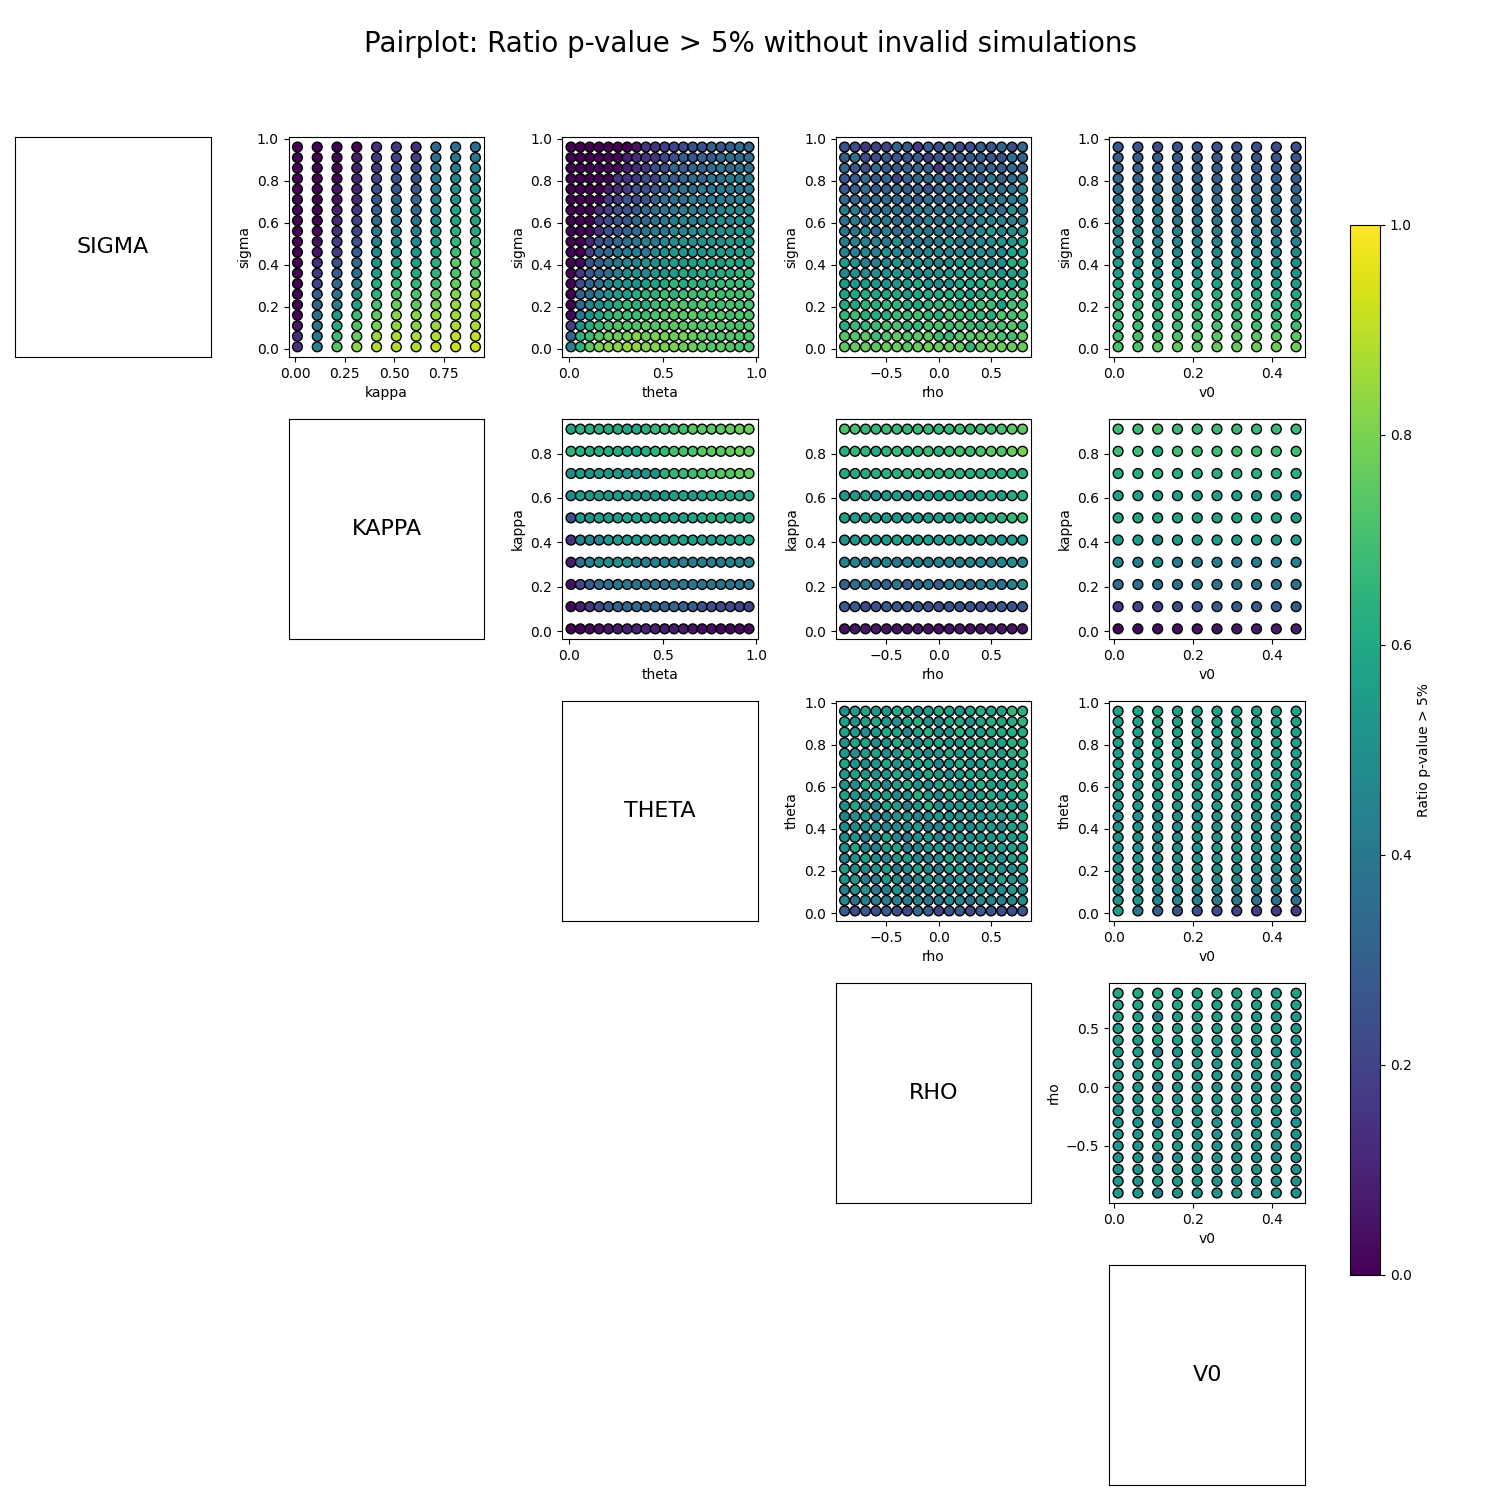
\includegraphics[width=0.8\textwidth]{img/pairplot_GC_cum_KS_muzero.png}
    \caption{Pairplot for each pair of parameters for the Heston Model and the percentage of p values of the Kolmogorov-Smirnov-Test for the Gram-Charlier Expansion with Cumulants vs the theoretical density above 5\%. Invalid simulations are excluded and $\mu=0$.}
    \label{fig:pairplot_GC_cum_KS_muzero}
\end{figure}

\begin{figure}
    \centering
    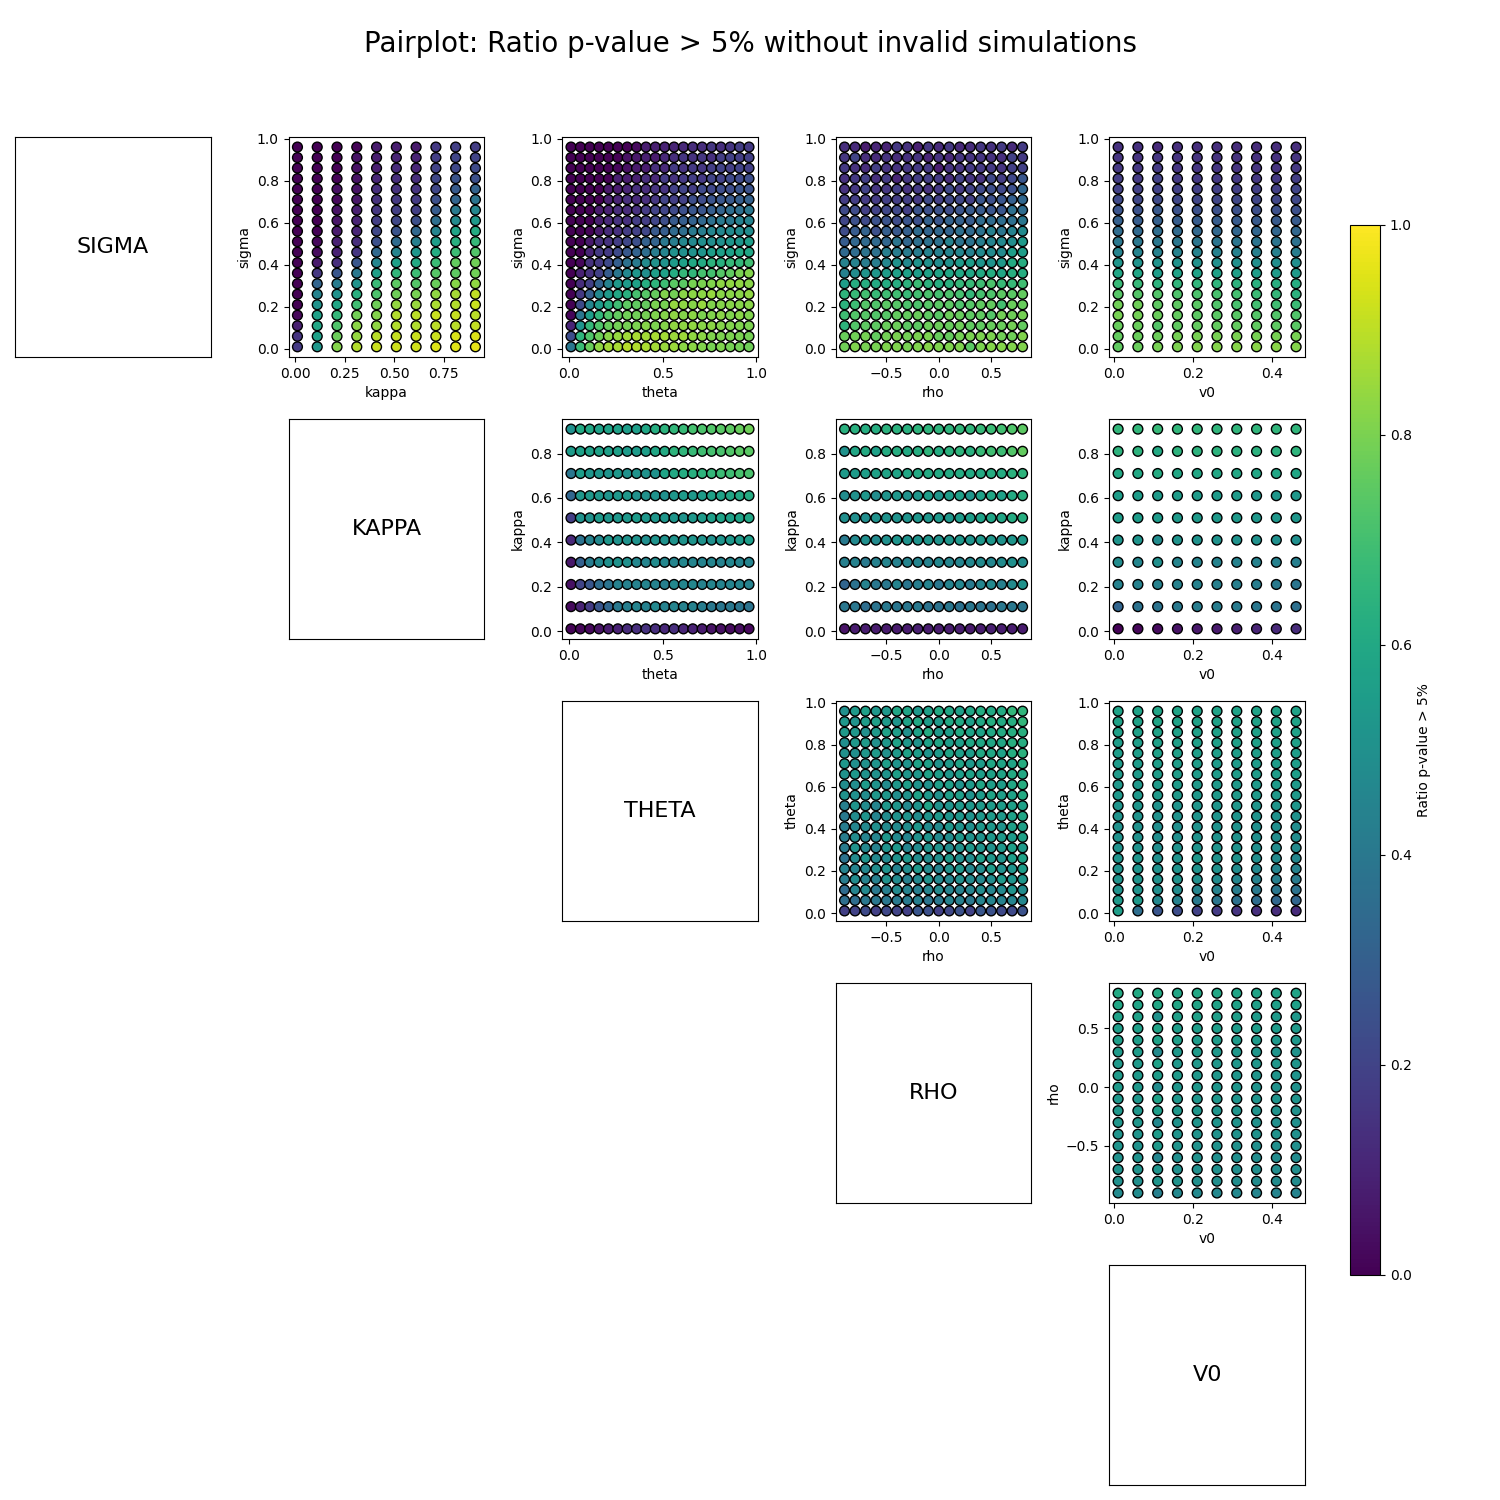
\includegraphics[width=0.8\textwidth]{img/pairplot_GC_cum_KS.png}
    \caption{Pairplot for each pair of parameters for the Heston Model and the percentage of p values of the Kolmogorov-Smirnov-Test for the Gram-Charlier Expansion with Cumulants vs the theoretical density above 5\%. Invalid simulations are excluded and $\mu=0.05$.}
    \label{fig:pairplot_GC_cum_KS_mu005}
\end{figure}

- Wir können schauen, wie sich der Pairplot Abbildung \ref{fig:pairplot_GC_cum_KS_muzero} ändert, wenn wir die Bedingung, dass der Preisprozess ein Martingale sein muss, verletzen. Dazu setzen wir $\mu=0.05$ und erhalten Abbildung \ref{fig:pairplot_GC_cum_KS_mu005}. Es fällt direkt auf, dass es weiße Stellen im Diagramm gibt. Das sind die Fälle, bei denen durch das Herausfiltern aller ungültigen Simulationen keine Simulationen mehr übrig bleiben. Das ist immer dann der Fall, wenn die Feller condition stark nicht erfüllt ist, also $2\kappa\theta - \sigma^2 <0$. Interessant ist, dass dieser Effekt nur bei $\mu=0.05$ so stark zum Tragen kommt, bei $mu=0$ fielen nicht so viele Simulationen weg.
- Der andere, sehr überraschende Punkt ist, dass es insgesamt mehr gelbe Punkte gibt, die Gram-Charlier-Expansion sich also -- für passend gewählte Parameter -- besser an die theoretische Dichte annähert, wenn der Preisprozess kein Martingale ist. Im Gegenzug gibt es aber auch mehr Parameterkombinationen (insbesondere $\sigma$, $\kappa$ und $\theta$), bei denen sich die Gram-Charlier-Expansion schlechter an die theoretische Dichte annähert.

\begin{figure}
    \centering
    \begin{subfigure}[b]{0.4\textwidth}
        \centering
        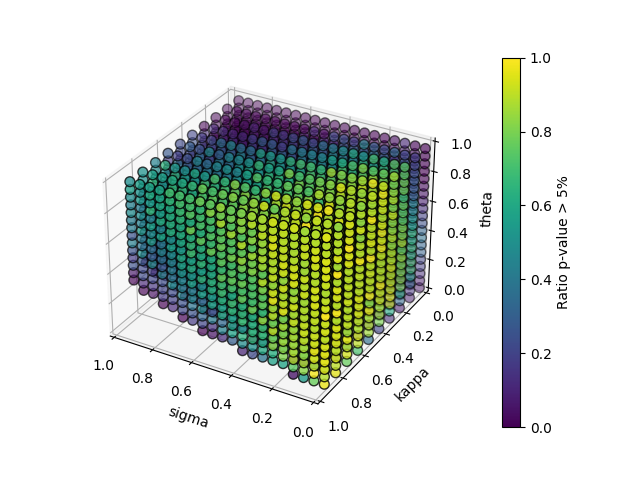
\includegraphics[width=\textwidth]{img/GC_cum_KS_3d_p_value_sigma_kappa_theta_muzero.png}
        \caption{$\mu=0$}
        \label{fig:GC_cum_KS_3d_p_value_sigma_kappa_theta_muzero}
    \end{subfigure}
    \hfill
    \begin{subfigure}[b]{0.4\textwidth}
        \centering
        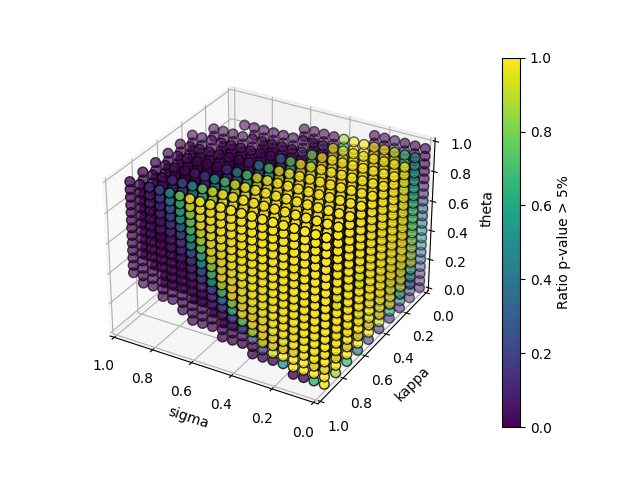
\includegraphics[width=\textwidth]{img/GC_cum_KS_3d_p_value_sigma_kappa_theta.png}
        \caption{$\mu=0.05$}
        \label{fig:GC_cum_KS_3d_p_value_sigma_kappa_theta}
    \end{subfigure}
    \caption{Percentage of simulations where the p-value of the Kolmogorov-Smirnov-Test against the theoretical density is above 5\%. Invalid simulations are excluded.}
    \label{fig:GC_cum_KS_3d}
\end{figure}

- In der detaillierteren Darstellung \ref{fig:GC_cum_KS_3d} sieht man besonders deutlich den Unterschied zwischen $mu=0$ (Abbildung \ref{fig:GC_cum_KS_3d_p_value_sigma_kappa_theta_muzero}) und $mu=0.05$ (Abbildung \ref{fig:GC_cum_KS_3d_p_value_sigma_kappa_theta}). Aus Gründen der Übersichtlichkeit wurde nicht noch eine Fläche eingezeichnet, ab wann die Feller condition erfüllt und nicht erfüllt ist, aber fast alle Punkte in Abbildung \ref{fig:GC_cum_KS_3d_p_value_sigma_kappa_theta} liegen innerhalb des Bereiches, in dem die Feller condition erfüllt ist, während es in Abbildung \ref{fig:GC_cum_KS_3d_p_value_sigma_kappa_theta_muzero} auch Punkte gibt, die außerhalb liegen. Es ist unklar, wie sich dieser Bereich charakterisieren lässt, die Feller condition bzw die Distanz $D$ reicht dafür nicht aus.

\subsection{Comparing the Tails with the Anderson-Darling-Test}

- Persönlich hätte ich vermutet, dass sich die Ergebnisse ändern, wenn man nun einen Test verwendet, der stärker auf die Ränder der Verteilung reagiert, wie den Anderson-Darling-Test. Aber man sieht, dass es praktisch keinen Unterschied zwischen den Abbildungen \ref{fig:pairplot_GC_cum_AD_muzero} + \ref{fig:pairplot_GC_cum_AD_mu005} und den Abbildungen \ref{fig:pairplot_GC_cum_KS_muzero} + \ref{fig:pairplot_GC_cum_KS_mu005} gibt.

\begin{figure}
    \centering
    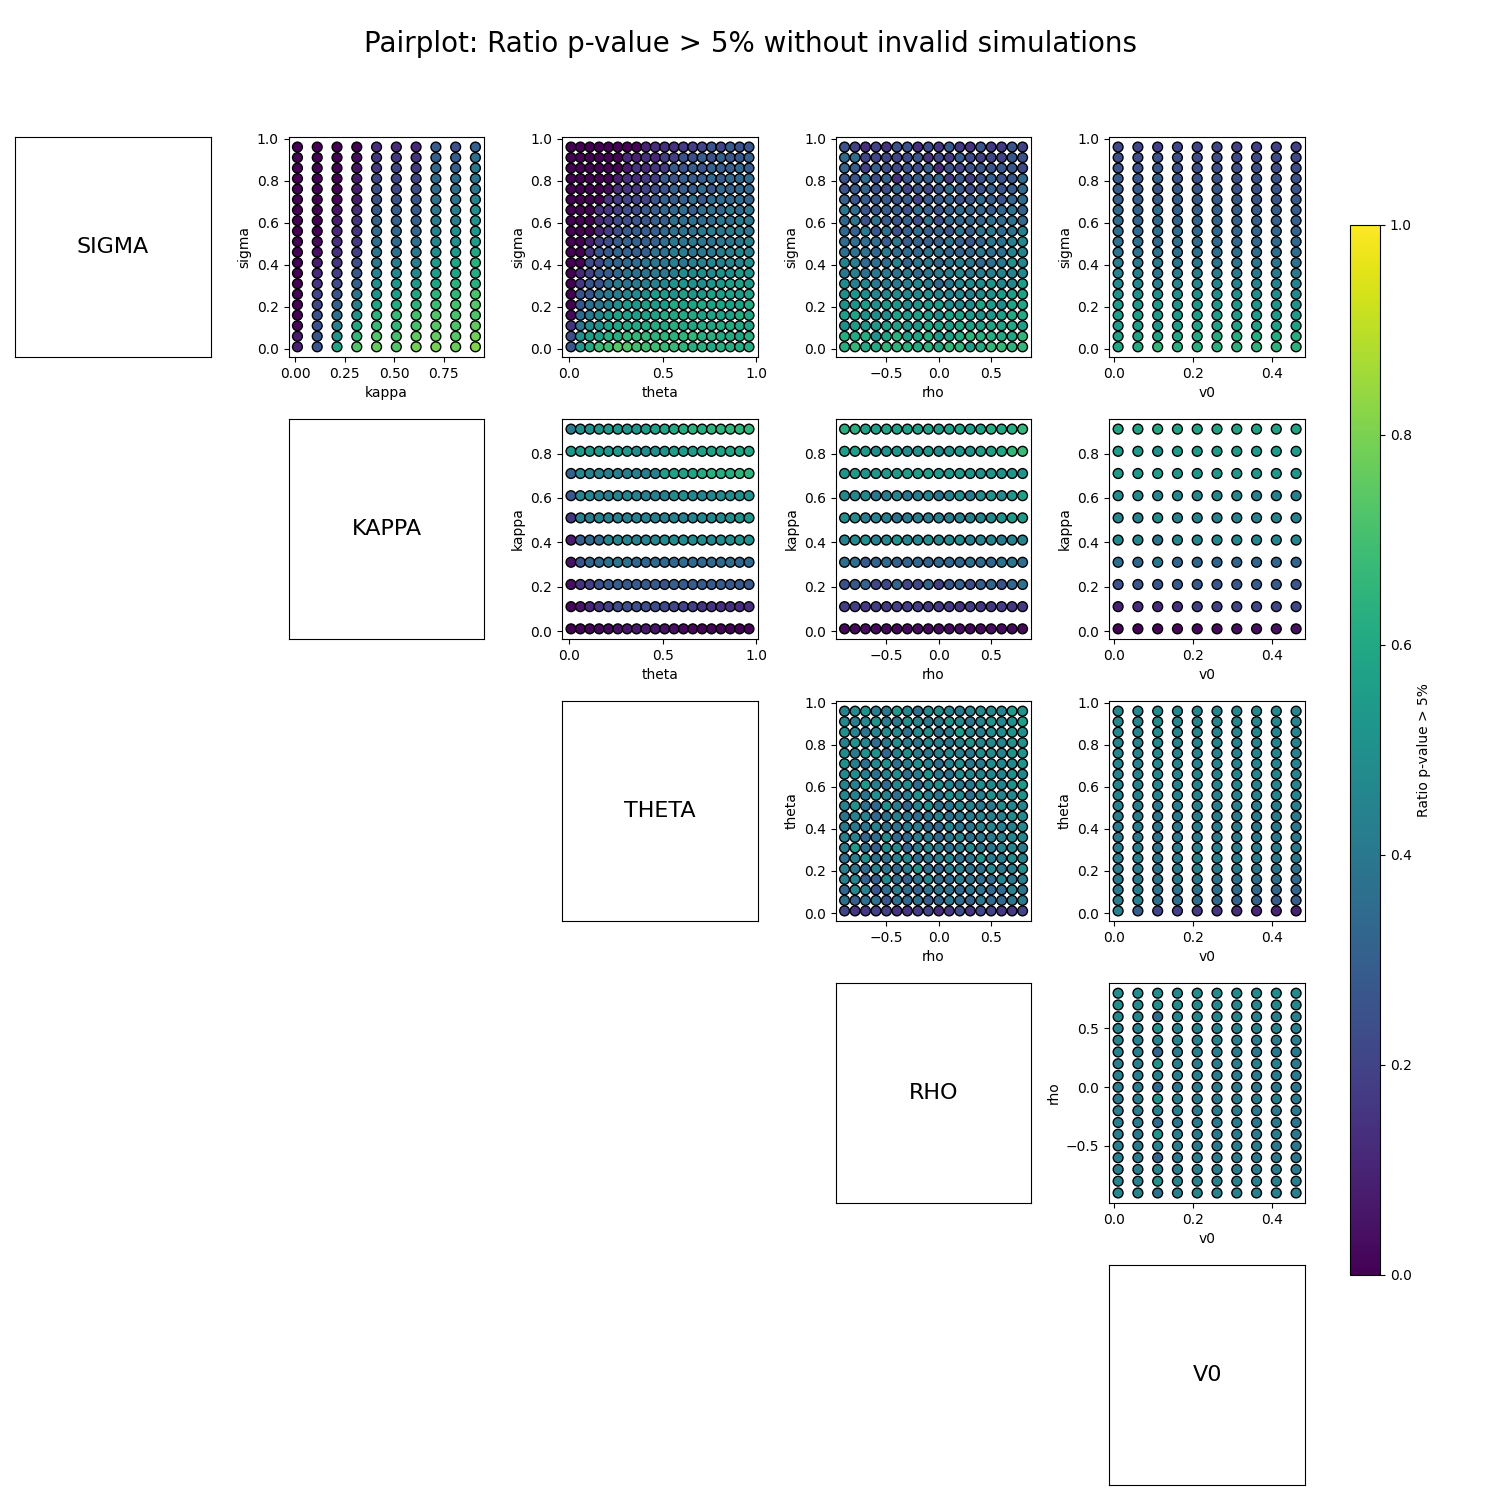
\includegraphics[width=0.8\textwidth]{img/pairplot_GC_cum_AD_muzero.png}
    \caption{Pairplot for each pair of parameters for the Heston Model and the percentage of p values of the Anderson-Darling-Test for the Gram-Charlier Expansion with Cumulants vs the theoretical density above 5\%. Invalid simulations are excluded and $\mu=0$.}
    \label{fig:pairplot_GC_cum_AD_muzero}
\end{figure}

\begin{figure}
    \centering
    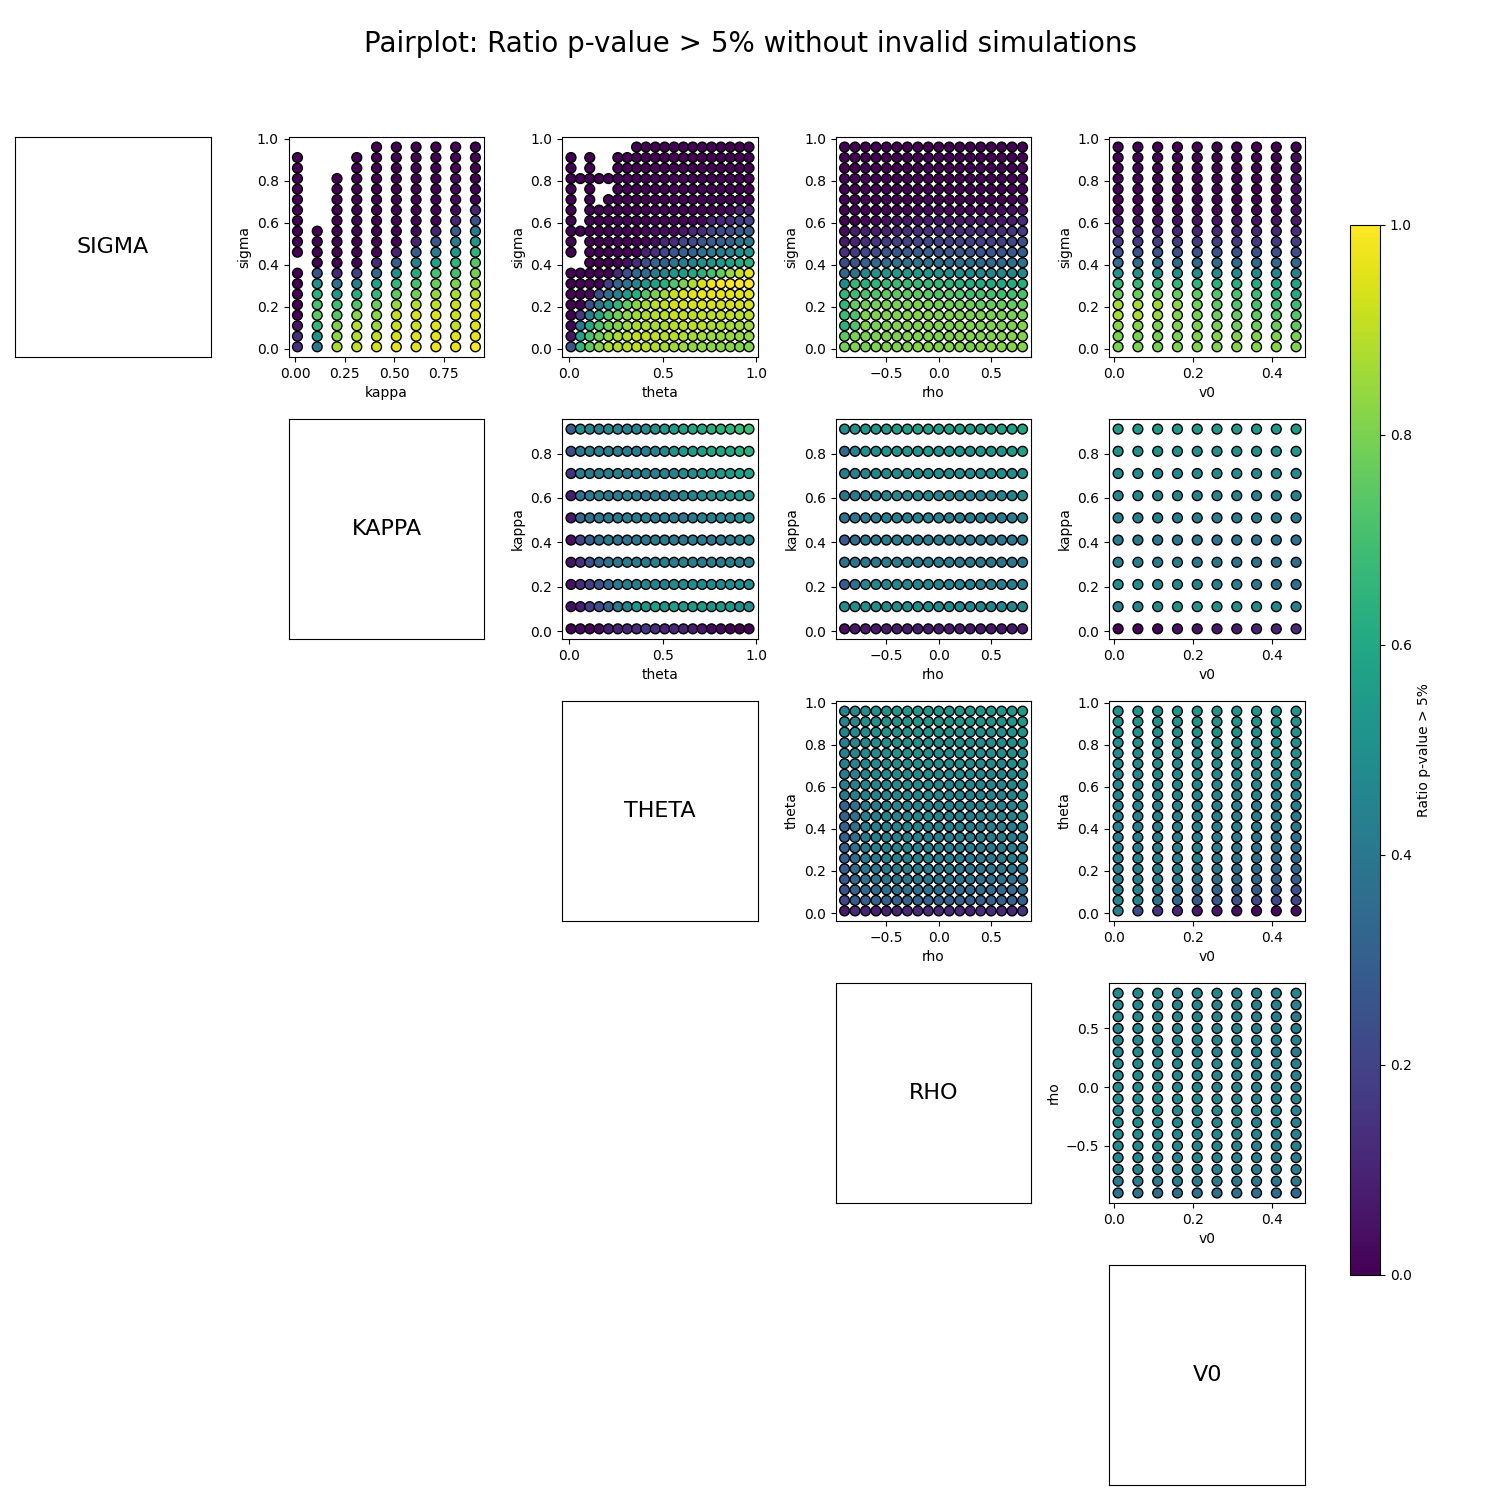
\includegraphics[width=0.8\textwidth]{img/pairplot_GC_cum_AD.png}
    \caption{Pairplot for each pair of parameters for the Heston Model and the percentage of p values of the Anderson-Darling-Test for the Gram-Charlier Expansion with Cumulants vs the theoretical density above 5\%. Invalid simulations are excluded and $\mu=0.05$.}
    \label{fig:pairplot_GC_cum_AD_mu005}
\end{figure}